%
% Exemple de rapport
% par Pierre Tremblay, Universite Laval
% modifié par Christian Gagne, Universite Laval
% 14/01/2011 - version 1.3
% modifié par Robert Bergevin, Université Laval
% 24/11/2011
% modifié par Jean-Yves Chouinard, Université Laval
% 11/01/2016
% modifié par Jean-Yves Chouinard, Université Laval
% 04/01/2017
%

%
% Modele d'organisation d'un projet LaTeX 
% rapport/      dossier racine et fichier principal
% rapport/fig   fichiers des figures
% rapport/tex   autres fichiers .tex
%

% ** Preambule **
%
% Ajouter les options au besoin :
%    - "ULlof" pour inclure la liste des figures, requis si "\begin{figure}" utilise
%    - "ULlot" pour inclure la liste des tableaux, requis si "\begin{table}" utilise
%
\documentclass[12pt,ULlof,ULlot]{ULrapport}

% Chargement des packages supplementaires (si absent de la classe)
\usepackage[utf8]{inputenc}
\usepackage[T1]{fontenc}
\usepackage[french]{babel}
%\usepackage[options]{nom_du_package}

% Definition d'une commande pour presenter des cellules multilignes dans un tableau
\newcommand{\cellulemultiligne}[1]{\begin{tabular}{@{}c@{}}#1\end{tabular}}

% Definition de colonnes en mode paragraphe avec alignement ajustable
% Cette definition requiert le chargement du package "array"
%    - alignement horizontal, parametre #1 : - \raggedright (aligne a gauche)
%                                            - \centering (centre)
%                                            - \raggedleft (aligne a droite)
%    - alignement vertical, parametre #2 : - p (aligne en haut)
%                                          - m (centre)
%                                          - b (aligne en bas)
%    - largeur, parametre #3 : longueur
\newcolumntype{Z}[3]{>{#1\hspace{0pt}\arraybackslash}#2{#3}}

% Definitions des parametres de la page titre
\TitreProjet{Grand Nord}                         % Titre du projet
\TitreRapport{Rapport de projet -- version 0}                       % Titre du rapport
\Destinataire{Robert Bergevin, Luc Lamontagne et Simon Thibault}         % Nom(s) du destinataire
\NumeroEquipe{2}                                     % Numero de l'equipe
\NomEquipe{NordFaune}                               % Nom de l'equipe
\TableauMembres{%                                     % Tableau des membres de l'equipe
   537\,393\,739  & Antoine Robert    &  8\\\hline        % matricule & nom & \\\hline
   537\,203\,820  & Mathis Carrier        & 1\\\hline        % matricule & nom & \\\hline
   537\,397\,278  & Felix-Antoine Guimont          & 6\\\hline        % matricule & nom & \\\hline
   537\,433\,045  & Louise Lesser   & 7\\\hline        % matricule & nom & \\\hline
   537\,294\,591  & Kayanne Loudiyi   & 4\\\hline        % matricule & nom & \\\hline
   537\,439\,306  & Phanuel Kouadio     & 3\\\hline        % matricule & nom & \\\hline
   537\,390\,654  & Louis-Charles Blais     & 2\\\hline        % matricule & nom & \\\hline
}
\DateRemise{29 janvier 2026}                           % Date de remis


% Contenu de l'historique des versions
\HistoriqueVersions{%                        % version & date & description \\\hline
         & 21 janvier 2026 & Création du document \\\hline
   1.0   & 29 janvier 2026 & Rédaction de l'introduction et du chapitre de la description.\\\hline
   }


% Corps du document

\begin{document}

%   Chapitres
%!TEX encoding = IsoLatin

%
% Chapitre "Introduction"
%

\chapter{Introduction}
\label{s:intro}

Grand Nord est un projet de d�veloppement d'un concept de capteur autonome fixe dans le but de compter ainsi que de documenter la faune arctique. Le Minist�re de la Faune Arctique nous sollicite donc pour construire ce syst�me autonome qui devra �chantillonner les activit�s des lemmings qui se trouvent sur le site arctique en recueillant, entre autres, des images et d'autres donn�es importantes de qualit�s dans le but de produire diverses statistiques. Le syst�me doit �tre robuste et fiable afin d'assurer une interaction externe minimale avec celui-ci advenant le cas d'un probl�me. Il devra aussi �tre en mesure de fonctionner de mani�re autonome pour une dur�e d'une ann�e. Finalement, il est important de prendre en consid�ration les co�ts li�s � la production de ce syst�me autonome et de pr�voir une installation facile ne moyennant pas de comp�tences en ing�nierie.

\bigskip
Ce rapport sera divis� en 6 chapitres afin de bien s�parer chaque concept concernant la mise en oeuvre de ce syst�me.
\begin{itemize}
   \item Description;
   \item Besoins et objectifs;
   \item Cahier des charges;
   \item Conceptualisation et analyse de faisabilit�;
   \item �tude pr�liminaire;
   \item Concept retenu.
\end{itemize}





%
% Chapitre "Structure d'un rapport technique"
%

\chapter{Description}
\label{s:description}

L'équipe d'ingénieurs de NordFaune a été mandatée afin de produire le design conceptuel d'un dispositif autonome fixe destiné à l'échantillonnage de la faune arctique. Cet équipement, conçu pour le Grand Nord, doit permettre l'échantillonnage des activités de lemmings évoluant sur un site arctique de façon complètement passive. Il doit être en mesure d'automatiser et de rendre la mesure autonome pour une période d'un an. 

\bigskip
Une première utilisation consiste à recueillir des images et à collecter les informations à des fins statistiques, tout en assurant une qualité constante des mesures. Ces données devront être archivées pour une période minimale d'au moins un an. La solution proposée vise également à documenter les statistiques sur le territoire tout en réduisant les coûts liés aux relevés terrain. Elle doit assurer une interaction externe minimale en cas de problème. 

\iffalse
\bigskip
L'installation doit permettre une communication hebdomadaire avec une centrale située à plus de 2000 km, offrir une console locale ainsi qu'une application mobile pour l'accès à distance, et fournir un accès sécurisé à la centrale pour trois personnes. Le dispositif devra également être capable de capturer des vidéos visibles ou en proche infrarouge (NIR) d'une durée minimale de 5 secondes, avec une résolution d'au moins 720p à 15 images par seconde. Le temps maximal entre deux vidéos est fixé à une heure. Les vidéos, les paramètres de configuration ainsi que les alarmes devront être conservés pour une période minimale d'un an. Une génération automatique d'alarmes devra être assurée lorsqu'une ou plusieurs fonctionnalités ne sont pas utilisables.
\fi 

\bigskip
Enfin, l'équipement devra être déployé dans un environnement nordique isolé tout en restant fonctionnel dans des conditions de température comprises entre -20 °C et +20 °C. De plus, il doit être fixé par le client, malgré un accès très limité au site. NordFaune doit donc proposer une solution fiable, durable et autonome afin de répondre au besoin de comptage et de documentation de la faune arctique.

%
% Chapitre "Structure d'un rapport technique"
%

\chapter{Besoins et objectifs}
\label{s:objectifs}
\section{Analyse des besoins}
Avant de se lancer dans la conception du projet et dans le but d'offrir au client le meilleur produit possible,
plusieurs besoin principaux ont été cernés. Premièrement, le système conceptualisé devra fonctionner de manière
complétement autonome. En effet, notre mandat exige que notre système devra être en mesure d'effectuer la prise
de données de manière complètement autonome pour une durée d'un an. À noter qu'il sera accessible selement pendant
2 semaine lors du mois de juin.

\bigskip
Deuxièmement, le système doit être robustre et doit être capable de supporter de gros écarts de température.
En effet, puisque ce système sera déployé dans l'artique québecois sur une période d'un an, il pourrait s'exposer
à des écarts de température pouvant varier entre -20°C et 20°C. De plus, le système devra être robustre et solide
afin d'être en mesure de fonctionner même si'il peut être recouvert par plus de 2 mètres de neige pendant une période
de 8 mois.

\bigskip
Troisièmement, le système devra limiter ses interactions avec la faune. Puisque ce dispositif sera potentiellement
installé dans des zones protégées, il devra assurer une mesure passive des données. En d'autres mots, il ne devra pas
piéger la faune afin de receuillir ses données. De plus\dots

\section{Analyse des objectif}
\section{Hiérarchisation des objects}

%
% Chapitre "Structure d'un rapport technique"
%

\chapter{Cahier des charges}
\label{s:cahier_des_charges}
\section{Automatisation du système}
\section{Installation}
\section{Coût de production}
%
% Chapitre "Structure d'un rapport technique"
%

\chapter{Conceptualisation}
\label{s:conceptualisation}
\section{Diagramme Fonctionnel}
Pour s'assurer de bien répondre aux demandes du client, nous devons tenir compte des intrants et extrants du système conceptualisé. Nous devons aussi penser à des fonctions qui permettront de faire le lien entre ce qui entre dans notre système et ce qui en ressortira. La figure \ref{diagramme_fonctionnel} est une représentation graphique des liens entre les intrants et extrants ainsi que les fonctions intermédiaires entre ceux-ci.

\begin{figure}[p]
    \centering
    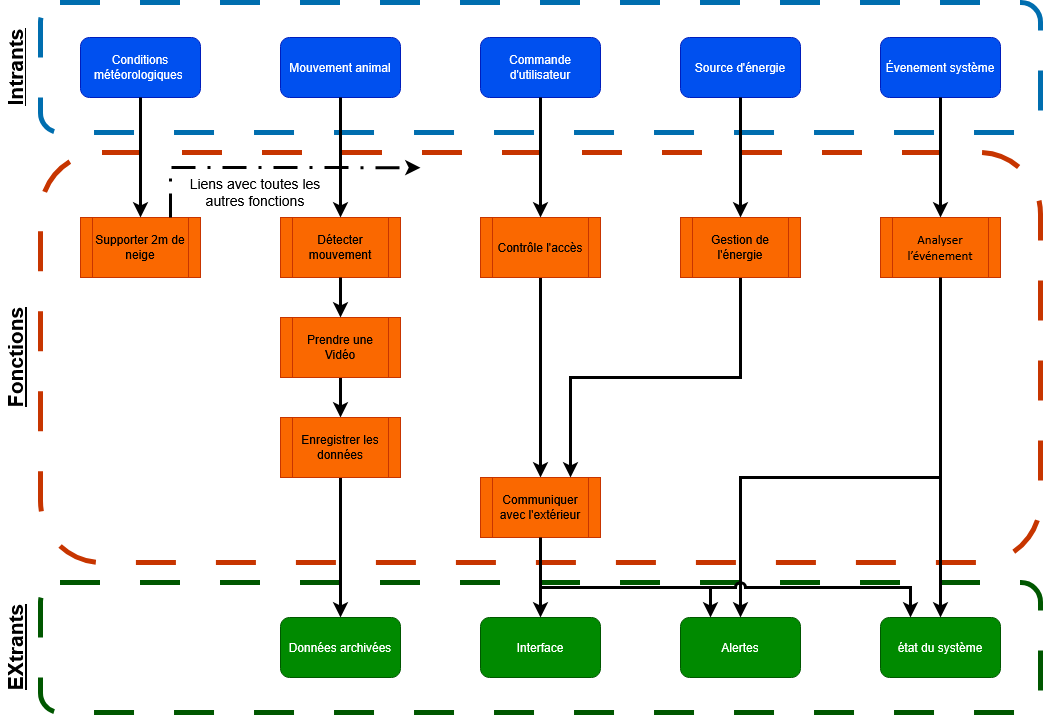
\includegraphics[width=1\textwidth]{fig/diagramme_fonctionnel.png}
    \caption{Diagramme fonctionnel du projet NordFaune}
    \label{diagramme_fonctionnel}
\end{figure}

\section{Conceptualisation des solutions}
\subsection{Prendre une vidéo}
La prise de vidéo est un concept capital du projet NordFaune, puisque les vidéos captées seront utilisées à des fins statiques par la suite. Il est donc important d'assurer une qualité constante de chaque vidéo, en s'assurant toutefois de ne pas dépasser les limites imposées par le système. (Voir \ref{} sur le stockage des données)
\bigskip

\textbf{Aspect physique:}
\begin{itemize}
    \item Le capteur vidéo doit être assez petit pour pouvoir être intégré au système.
    \item Les vidéos captées par l'appareil doivent disposer d'une résolution satisfaisante pour une analyse future.
    \item Doit pouvoir communiquer et interagir avec un ordinateur moderne.
\end{itemize}

\textbf{Aspect économique:}
\begin{itemize}
    \item Le capteur doit être peut couteux.
\end{itemize}

\textbf{Aspect temporel:} N/A

\textbf{Aspect socio-environnemental:}
\begin{itemize}
    \item Ne doit pas interférer avec la faune artique.
\end{itemize}

\subsubsection{GoPro Hero}
\textbf{Description} La caméra Hero de la marque GoPro est une petite caméra très compacte et légère. (56,6 mm de large et 29,4 mm de hauteur) Elle peut enregistrer des vidéos jusqu'à une résolution de 4k à 30 FPS et dispose d'un port microSD pour pouvoir enregistrer les vidéos capturées. Au besoin, elle peut se connecter VIA Wifi, Bluetooth ou tout simplement à l'aide d'un câble USB-C  pour communiquer et transférer ses données vers un ordinateur. La caméra Hero est robuste et étanche jusqu'à une profondeur de 5m. De plus, elle résiste généralement bien au froid, surtout si connectée à une source d'énergie externe. La caméra Hero peut s'acheter facilement sur le site de GoPro ou sur Amazon à un prix d'environ 280\$.

\textbf{Décision} Rejetée

\textbf{Justification} Ce concept a été rejeté, puisque malgré plusieurs caractéristiques intéressantes comme la robustesse et l'étanchéité, le prix de 280\$ est tout simplement trop élevé. De plus, plusieurs caractéristiques de cette caméra sont tout simplement inutiles pour la mise en œuvre du design conceptuel. C'est le cas de la captation vidéo jusqu'à une résolution de 4k qui demande beaucoup d'espace de stockage et qui n'est pas nécessaire pour une bonne analyse des images.

\textbf{Références}
\cite{Gopro1}
\cite{Gopro2}

\subsubsection{ArduCam IMX219}
\textbf{Description} La caméra ArduCam IMX219 est principalement conçue pour permettre une intégration facile avec les ordinateurs Raspberry Pi. Avec son capteur de 8MP, il est possible de prendre des vidéos HD jusqu'à 47 images par seconde. Le module communique directement avec un ordinateur Raspberry Pi par l'intermédiaire de deux lignes MIPI CSI-2. Elle est très compacte et elle sera facile à installer dans la boîte avec les autres composants du système. De plus, puisque c'est seulement un module de caméra dédié uniquement à la prise de photos ou de vidéos, il consomme très peu d'énergie. Avec un prix de 30\$ dur le site de ArduCam ou 40\$ sur Amazon, cette caméra n'est pas dispendieuse et facile à se procurer.

\textbf{Décision} Retenue

\textbf{Justification} Ce concept est retenu, puisqu'il répond aisément à tous les critères. Il n'est pas cher, occupe très peu d'espace et peut enregistrer des vidéos avec une résolution acceptable. Cependant, il est préférable d'utiliser un ordinateur Raspberry avec ce capteur ce qui facilitera son installation et sa mise en marche.

\textbf{Références} 
\cite{Gopro1}
\cite{Gopro2}
%
% Chapitre "Structure d'un rapport technique"
%

\chapter{Étude préliminaire}
\label{s:etude_preliminaire}
\section{Plan de développement}
Afin d'asurer une évaluation systématique de chaque concept, un plan d'étude a été élaboré.
Le tableau \ref{tab:plan_etude} présente en détail la procédure d'évaluation de chacun des critères, appliqué aux trois concepts exposés dans le tableau \ref{tab:concepts_nordfaune}.


\newcolumntype{L}[1]{>{\RaggedRight\arraybackslash}p{#1}}
\renewcommand{\arraystretch}{1.4}

\begin{longtable}{|L{4cm}|L{6cm}|L{6cm}|}
\caption{Plan d'étude pour les différents critères}
\label{tab:plan_etude} \\

\hline
\textbf{Critères} & \textbf{Procédures} & \textbf{Hypothèses} \\
\hline
\endfirsthead

\multicolumn{3}{c}{\textit{Table 6.1 -- (suite)}} \\
\hline
\textbf{Critères} & \textbf{Procédures} & \textbf{Hypothèses} \\
\hline
\endhead

% ------------- LIGNES -------------

\ref{robutesse_autonomie} Marge de l'état d'autonomie
    & Évaluer l'autonomie la plus basse du système selon les données du fournisseur.
    & Toutes les composantes fonctionnent dans leurs plages nominales.
\\
\hline

\ref{consommation_electrique} Consommation énergétique
    & Évaluer la somme des consommation électrique selon les données du fournisseur.
    & Le système fonctionne de manière continue sous conditions climatiques normales.
\\
\hline

\ref{resilience_systeme} Proportion des fonctions protégées
    & Évaluer le nombre de fonctions protégées par la redondance ou une mesure de protection.
    & Chaque fonction critique peut être protégée indépendamment.
\\
\hline

\ref{conditions_climatiques} Plage opérationnelle de température
    & Évaluer la température minimale d'opération selon les données du fournisseur.
    & L'isolation thermique du système est uniforme et stable.
\\
\hline

\ref{installation_deploiement} Encombrement et complexité d'installation 
    & Évaluer le volume du sytème et sa manipulation selon les données du fournisseur.
    & La forme du système est manipulable par deux personnes.
\\
\hline

\ref{resistance_neige} Résistance mécanique à la neige 
    & Évaluer la charge maximale supportée par le boîtier selon les données du fournisseur.
    & La neige est répartie uniformément sur le boîtier.
\\
\hline

\ref{detection_mammiferes} Couverture de la zone d'observation
    & Évaluer par projection géométrique la proportion de l'aire couverte.
    & Les capteurs ne sont pas obstrués et sont placés à l'endroit optimal.
\\
\hline

\ref{conservation_donnees} Capacité de stockage
    & Évaluer à partir de l'encodage, la fréquence, la durée et la résolution de la capture.
    & La compression et le format sont constants et uniformes.
\\
\hline

\ref{performance_communication} Performance de communication distante
    & Évaluer la portée maximale selon les données du fournisseur.
    & La ligne de communication n'a aucun obstacles majeurs.
\\
\hline

\ref{exploitation_scientifique} Qualité scientifique des données
    & Évaluer la fréquence d'image que l'appareil de capture offre selon le fabricant.
    & Les capteurs vidéo fonctionne à cadence régulière.
\\
\hline

\ref{impact_lumineux} Impact lumineux sur la faune
    & Évaluer avec la longueur d'onde de la lumière visible produite.
    & Les lemmings ne sont sensibles qu'à la lumière dans la plage définie.
\\
\hline

\ref{impact_environnemental} Impact environnemental
    & Évaluer le nombre de batteries consommées annuellement selon le fournisseur.
    & Chaque batterie a une autonomie prévisible.
\\
\hline

\ref{couts_transport} Coûts d'installation et de transport
    & Évaluer en fonction de la somme des frais d'installation des éléments cruciaux.
    & Les coûts de transport et d'installation sont proportionnels au temps exigé.
\\
\hline

\ref{couts_entretien} Coûts d'opération et d'entretien
    & Évaluer selon le coûts du renouvellement des mesures de protection, les frais qu'apporte l'opération et d'autres coûts obligatoires.
    & Les frais récurrents sont stables.
\\
\hline

\ref{couts_fabrication} Coûts de fabrication
    & Évaluer avec la somme des coûts des composantes majeures à l'achat.
    & Les prix des composants sont constants et correspondent aux prix affichés.
\\
\hline

\end{longtable}


\renewcommand{\arraystretch}{1.5}

\begin{table}[htp]
\centering
\caption{Les trois concepts pour le projet NordFaune}
\label{tab:concepts_nordfaune}

\begin{tabular}{|L{6cm}|L{3cm}|L{3cm}|L{3cm}|}
\hline
\textbf{Fonctions} & \textbf{Concept 1} & \textbf{Concept 2} & \textbf{Concept 3} \\
\hline

% ------------- LIGNES -------------

\ref{CapturerUneVidéo} Capturer une vidéo
    & \hyperref[sec:arduc]{ArduCam IMX219}
    & \hyperref[sec:gopro]{GoPro Hero}
    & \hyperref[sec:esp32]{ESP32-CAM}
\\
\hline

\ref{DétecterLeMouvement} Détecter le mouvement
    & \hyperref[sec:plaque]{Plaque piézoélectriques}
    & \hyperref[sec:capte]{Capteur infrarouge}
    & \hyperref[sec:capte]{Capteur infrarouge}
\\
\hline

\ref{ContrôlerLAccès} Contrôler l'accès
    & \hyperref[sec:tunne]{Tunnel Cloudflare}
    & \hyperref[sec:micro]{Microsoft Authentificator}
    & \hyperref[sec:tunne]{Tunnel Cloudflare}
\\
\hline

\ref{EnregistrerDesDonnées} Enregistrer des données
    & \hyperref[sec:cartesd]{MicroSD(HC)}
    & \hyperref[sec:ssd]{SSD SATA III}
    & \hyperref[sec:azsta]{Azure et Starlink}
\\
\hline

\ref{DétecterUnÉnévement} Détecter un événement et l'état du système
    & \hyperref[sec:raspb]{Raspberry Pi}
    & \hyperref[sec:nano]{Nvidia Jetson Nano}
    & \hyperref[sec:raspb]{Raspberry Pi}
\\
\hline

\ref{RésisterAuxConditions} Résister aux conditions climatiques
    & \hyperref[sec:bois]{Bois de cèdre}
    & \hyperref[sec:alumi]{Aluminium}
    & \hyperref[sec:alumi]{Aluminium}
\\
\hline

\ref{GérerLÉnergie} Gérer l'énergie
    & \hyperref[sec:bloc]{Bloc de batteries}
    & \hyperref[sec:hybri]{Solution hybride}
    & \hyperref[sec:bloc]{Bloc de batteries}
\\
\hline

\ref{CommuniquerAvecExt} Communiquer avec l'extérieur
    & \hyperref[sec:iridi]{Iridium 9603 SBD}
    & \hyperref[sec:starl]{Starlink Performance}
    & \hyperref[sec:iridi]{Iridium 9603 SBD}
\\

\hline
\end{tabular}
\end{table}


\section{Élaboration et évaluation des concepts de solution}

% ------------- Concept #1 -------------

\subsection{Concept \#1 : Équilibre global}

Pour ce concept, les composantes ont été choisies de façon à garder un bon équilibre dans l'ensemble des fonctions du système, sans trop dépenser.

\subsubsection{Fonctionnement autonome du système}

\paragraph{Marge de l'état d'autonomie :}
Étant donné que ce concept utilise un contrôleur Raspberry Pi, une caméra ArduCam IMX219 et un module Iridium 9603 SBD, la consommation du système demeure modérée.
Le système se repose complètement sur les blocs de batteries non rechargeables, qui vont s’épuiser avant la durée de vie des composants électroniques.

\bigskip
La contrainte du client exige une autonomie minimale de douze mois.
Il est entièrement possible d’atteindre cette attente avec une quantité de batteries proportionnelle à la consommation.
Le facteur limitant est donc la capacité totale des batteries embarquées.
Alors, avec un dimensionnement optimisé (Voir \hyperref[par:encombrement]{Encombrement}), l’autonomie maximale du concept est estimée à environ 12,5 mois.
D’après le barème de la section \ref{robutesse_autonomie}, cette solution obtient une note de 0,29 pour ce concept, soit 2,9\% avec pondération.


\paragraph{Consommation énergétique :}
Texte

\paragraph{Proportion des fonctions protégées :}
Texte


\subsubsection{Résistance et entretien du système}

\paragraph{Plage opérationnelle de température :}
Texte

\paragraph{Encombrement et complexité d'installation :}
\label{par:encombrement}
Texte

\paragraph{Résistance mécanique à la neige :}
Texte


\subsubsection{Observation et gestion de données}

\paragraph{Couverture de la zone d'observation :}
Texte

\paragraph{Capacité de stockage :}
Texte

\paragraph{Performance de communication distante :}
Texte

\paragraph{Qualité scientifique des données :}
Texte


\subsubsection{Réduire impacts et coûts}

\paragraph{Impact lumineux sur la faune :}
Texte

\paragraph{Impact environnemental :}
Texte

\paragraph{Coûts d'installation et de transport :}
Texte

\paragraph{Coûts d'opération et d'entretien :}
Texte

\paragraph{Coûts de fabrication :}
Texte

% ------------- Concept #2 -------------

\subsection{Concept \#2 : Performance maximale}

Pour ce concept, les options les plus performantes ont été privilégiées pour garantir la meilleure performance, peu importe le coût.

\subsubsection{Fonctionnement autonome du système}

\paragraph{Marge de l'état d'autonomie :}
L’obtention d’une performance maximale apporte des composants très énergivores.
Une GoPro, un Nvidia Jetson Nano et un système Starlink ont une demande énergétique trop grande pour dépendre sur un système énergétique standard.
Alors, le concept exige la solution hybride combinant des batteries au Lithium-Thionyl Chloride et des condensateurs hybrides au lithium.
\bigskip

Le facteur limitant devient la durée maximale de vie planifiée lors de la conception des batteries $\mathrm{Li{-}SOCl_2}$.
Dans un circuit soumis à une très forte utilisation, elles sont capables d’atteindre une durée de 12 mois.
Nous estimons que, pour notre système qui utilise moins d’énergie que la valeur nominale, l’autonomie peut être assurée jusqu’ à 14 mois indépendamment des conditions externes.
Selon l’équation \ref{robutesse_autonomie}, le concept obtient donc une note de 0,79, ce qui correspond à un pourcentage de 7,9\%.


\paragraph{Consommation énergétique :}
Texte

\paragraph{Proportion des fonctions protégées :}
Texte


\subsubsection{Résistance et entretien du système}

\paragraph{Plage opérationnelle de température :}
Texte

\paragraph{Encombrement et complexité d'installation :}
Texte

\paragraph{Résistance mécanique à la neige :}
Texte


\subsubsection{Observation et gestion de données}

\paragraph{Couverture de la zone d'observation :}
Texte

\paragraph{Capacité de stockage :}
Texte

\paragraph{Performance de communication distante :}
Texte

\paragraph{Qualité scientifique des données :}
Texte


\subsubsection{Réduire impacts et coûts}

\paragraph{Impact lumineux sur la faune :}
Texte

\paragraph{Impact environnemental :}
Texte

\paragraph{Coûts d'installation et de transport :}
Texte

\paragraph{Coûts d'opération et d'entretien :}
Texte

\paragraph{Coûts de fabrication :}
Texte

% ------------- Concept #3 -------------

\subsection{Concept \#3 : Durabilité à long terme}

Pour ce concept, les solutions les plus durables ont été sélectionnées afin d'assurer un bon fonctionnement à long terme.

\subsubsection{Fonctionnement autonome du système}

\paragraph{Marge de l'état d'autonomie :}
Étant donné que le concept est composé d’une ESP32-CAM, d’un Raspberry Pi et d’un module Iridium 9603 SBD, la demande énergétique du système est fortement réduite.
L’alimentation est assurée par un bloc de batteries optimisé.
\bigskip

Dans ce cas, le facteur limitant est plutôt la durée de vie maximale des composants électroniques, notamment le module ESP32-CAM et le module Iridium, qui ont une fiabilité réduite lors d’une utilisation sur une longue période dans des conditions extrêmes.
L’autonomie est estimée comme étant assurée pendant 18 mois.
Cette durée lui donne une note de 1 selon l’équation \ref{robutesse_autonomie}, ce qui correspond à un pourcentage de 10\%.


\paragraph{Consommation énergétique :}
Texte

\paragraph{Proportion des fonctions protégées :}
Texte


\subsubsection{Résistance et entretien du système}

\paragraph{Plage opérationnelle de température :}
Texte

\paragraph{Encombrement et complexité d'installation :}
Texte

\paragraph{Résistance mécanique à la neige :}
Texte


\subsubsection{Observation et gestion de données}

\paragraph{Couverture de la zone d'observation :}
Texte

\paragraph{Capacité de stockage :}
Texte

\paragraph{Performance de communication distante :}
Texte

\paragraph{Qualité scientifique des données :}
Texte


\subsubsection{Réduire impacts et coûts}

\paragraph{Impact lumineux sur la faune :}
Texte

\paragraph{Impact environnemental :}
Texte

\paragraph{Coûts d'installation et de transport :}
Texte

\paragraph{Coûts d'opération et d'entretien :}
Texte

\paragraph{Coûts de fabrication :}
Texte



\section{Synthèse des résultats}
Le tableau \ref{tab:synth} présente les valeurs obtenues pour chaque critère en fonction des différents concepts.
Ces valeurs permettent ensuite de calculer la note obtenue à l'aide des barèmes du \hyperref[s:cahier_des_charges]{cahier des charges}.

\begin{table}[h!]
\centering
\caption{Synthèse des résultats}
\label{tab:synth}
\renewcommand{\arraystretch}{1.2}
\begin{tabularx}{\textwidth}{|X|c|c|c|}
\hline
\textbf{Critères d'évaluation} & \textbf{Concept 1} & \textbf{Concept 2} & \textbf{Concept 3} \\
\hline

\textbf{\ref{Autonomie} Fonctionnement autonome du système} & & &  \\
\hline
\ref{robutesse_autonomie} Marge de l'état d'autonomie [mois] & 12,5 & 14 & 18 \\
\ref{consommation_electrique} Consommation énergétique [W] & & & \\
\ref{resilience_systeme} Proportion des fonctions protégées & & & \\
\hline

\textbf{\ref{Robustesse} Résistance et entretien du système} & & &  \\
\hline
\ref{conditions_climatiques} Plage opérationnelle de température [°C] & & & \\
\ref{installation_deploiement} Encombrement et complexité d’installation [$m^3$] & & & \\
\ref{resistance_neige} Résistance mécanique à la neige [$kg/m^2$] & & & \\
\hline

\textbf{\ref{donnees} Observation et gestion de données} & & & \\
\hline
\ref{detection_mammiferes} Couverture de la zone d’observation [\%] & & & \\
\ref{conservation_donnees} Capacité de stockage [Go] & & & \\
\ref{performance_communication} Performance de communication distante [km] & & & \\
\ref{exploitation_scientifique} Qualité scientifique des données [fps] & & & \\
\hline

\textbf{\ref{impacts_couts} Réduire impacts et coûts} & & &  \\
\hline
\ref{impact_lumineux} Impact lumineux sur la faune [nm] & & & \\
\ref{impact_environnemental} Impact environnemental & & & \\
\ref{couts_transport} Coûts d'installation et de transport [\$] & & & \\
\ref{couts_entretien} Coûts d'opération et d’entretien [\$] & & & \\
\ref{couts_fabrication} Coûts de fabrication [\$] & & & \\
\hline

\end{tabularx}
\end{table}

%
% Chapitre "Structure d'un rapport technique"
%

\chapter{Concept retenu}
\label{s:concept_retenu}
\section{Matrice de décision}
Texte

\section{Analyse de la matrice décisionnelle}
Texte

\begin{table}[h!]
\centering
\caption{Matrice décisionnelle}
\label{tab:matricede}
\small
\begin{tabular}{|l|c||c|c|c|}
\hline
Critères d'évaluation & Pond. & Concept 1 & Concept 2 & Concept 3 \\
\hline\hline
\textbf{\ref{Autonomie} Fonctionnement autonome du système} & \textbf{30\%} & & &  \\
\hline
\ref{robutesse_autonomie} Marge de l'état d'autonomie & 10\% & 2,9\% & 7,9\% & 10\% \\
\ref{consommation_electrique} Consommation énergétique & 8\% & 5\% & 0\% & 4,25\% \\
\ref{resilience_systeme} Proportion des fonctions protégées & 6\% & 3,6\% & 2,4\% & 4,8\% \\
\hline

\textbf{\ref{Robustesse} Résistance et entretien du système} & \textbf{30\%} & & &  \\
\hline
\ref{conditions_climatiques} Plage opérationnelle de température & 10\% & 0\% & 0\% & -30 \\
\ref{installation_deploiement} Encombrement et complexité d'installation & 6\% & 4,8\% & ?? & ?? \\
\ref{resistance_neige} Résistance mécanique à la neige & 12\% & 12\% & 12\% & 12\% \\
\hline

\textbf{\ref{donnees} Observation et gestion de données} & \textbf{25\%} & & & \\
\hline
\ref{detection_mammiferes} Couverture de la zone d'observation & 9\% & 9\% & 9\% & 93 \\
\ref{conservation_donnees} Capacité de stockage & 5\% & 0\% & 5\% & 134 \\
\ref{performance_communication} Performance de communication distante & 6\% & 5,1\% & ?? & ?? \\
\ref{exploitation_scientifique} Qualité scientifique des données & 5\% & 3,75\% & ?? & ?? \\
\hline

\textbf{\ref{impacts_couts} Réduire impacts et coûts} & \textbf{15\%} & & &  \\
\hline
\ref{impact_lumineux} Longueur d'onde de l'éclairage & 3\% & 3\% & 2,07\% & ?? \\
\ref{impact_environnemental} Nombre de remplacements de batterie par an & 2\% & 1,5\% & 2 & 1 \\
\ref{couts_transport} Coûts d'installation et de transport & 4\% & 3,1\% & 2000 & 2200 \\
\ref{couts_entretien} Coûts d'opération et d'entretien & 3\% & 1,97\% & 1500 & 1800 \\
\ref{couts_fabrication} Coûts de fabrication & 3\% & 2,58\% & 1500 & 2169 \\
\hline\hline

\textbf{Total} & \textbf{100\%} & & & \\
\hline
\end{tabular}
\end{table}

\section{Description du concept retenu}
\textbf{Sopporter les conditions métérologiques}
\begin{itemize}
    \item Protection du système avec un boitier en bois
\end{itemize}

\textbf{Détection d'un mouvement et enregistrement de vidéos}
\begin{itemize}
    \item La détection de mouvement sera assurée par des plaques piézoélectriques
    \item Les vidéos seront capturées par l'ArduCam IMX219
    \item Les données seront enregistrées sur une carte MicroSD(HC)
\end{itemize}

\textbf{Interface utilisateur}
\begin{itemize}
    \item Le système pourra être accédé par l'intermédiare du Tunnel Cloudflare
    \item La communication entre le système et l'extérieur sera assurée par l'Iridium 9603 SBD
\end{itemize}

\textbf{Gestion de l'énergie}
\begin{itemize}
    \item Le système sera alimenté par un blocs de batteries au Lithium-thionyl chloride
\end{itemize}

\subsection{Gestion de l'énergie}
L'entièreté du système sera alimenté par le bloc de batteries au Lithium-thionyl chloride.
Ces batteries hautes densistés combinées avec un système qui consomme au maximum 11.3 Watts pour
de très courtes pédiodes lors d'enregistrement vidéos, assurera une autonomie d'au moins 12 mois
pour le système.

Si l'on programme un système qui s'active uniquement lorsqu'un signal est envoyé par la plaque 
de pression, on peut estimer une consommation maximale en veille de 0,1 W, l'on garde la 
plaque piézoélectrique active. Avec une consommation 

\section{Conclusion}
Texte
%
% Chapitre "Bibliographie"
%

\begin{thebibliographyUL}{99} % remplacer le "{9}" par "{99}" lorsque le nombre de references
                              % requiert 2 caracteres (>= 10 references)%
    \bibitem{Gopro1} GoPro. GoPro HERO — Notre plus petite caméra d'action, [En ligne]. \url{https://gopro.com/fr/ca/shop/cameras/learn/hero/CHDHF-131-master.html} (Page consultée le 15 mars 2026)
    \bibitem{Gopro2} Amazon Canada. GoPro Hero — Caméra d'action compacte étanche avec vidéo 4K Ultra HD, photo 12 MP, écran tactile, [En ligne]. \url{https://www.amazon.ca/-/fr/GoPro-Hero-daction-compacte-étanche/dp/B0DCLRRHSP} (Page consultée le 15 mars 2026)
    \bibitem{ArduCam1} Amazon Canada. Arducam Module caméra 8MP IMX219, [En ligne]. \url{https://www.amazon.ca/Arducam-IMX219-Camera-Module-NVIDIA/dp/B082NVPC1N} (Page consultée le 15 mars 2026)
    \bibitem{ArduCam2} Arducam Wiki (2025). ArduCam Raspberry Pi Camera Module datasheet, [En ligne]. \url{https://docs.arducam.com/Raspberry-Pi-Camera/Native-camera/8MP-IMX219/} (Page consultée le 15 mars 2026)
    \bibitem{ArduCam3} ArdumCam.ca. 8MP IMX219 Camera Module for Raspberry Pi, [En ligne]. \url{https://www.arducam.com/8mp-imx219-camera-module-for-raspberry-pi-b0394.html} (Page consulteé le 15 mars 2026)
    \bibitem{ESP32-Cam1} Amazon Canada. Taidacent ESP32 Cam OV2640 Module de caméra, [En ligne]. \url{https://www.amazon.ca/Taidacent-OV2640-Megapixel-Interface-Breakout/dp/B08FJB4DJP} (Page consulteé le 15 mars 2026)
    \bibitem{ESP32-CAM2} Waveshare. ESP32-CAM, Camera Module Based On ESP32, OV2640 Camera and ESP32-CAM-MB adapter Included, Waveshare, Share Awesome Hardware, [En ligne]. \url{https://www.waveshare.com/ESP32-CAM.htm} (Page consulteé le 15 mars 2026)
    \bibitem{ESP32-CAM3} OmniVision Technologies, Inc. (2006, 28 février). OV2640 Color CMOS UXGA (2.0 MegaPixel) CameraChip — Preliminary Datasheet (Version 1.6), [Fiche technique]. \url{https://www.uctronics.com/download/cam_module/OV2640DS.pdf?srsltid=AfmBOoqS27skFVumXUpf3_LWmmNrdHi8q6Lqte7E42odDxsqJID3XElR} (Page consulteé le 15 mars 2026)
    \bibitem{CarteMicroSD1} Canada Computers, Kingston 8GB Industrial Temperature microSDHC UHS-I Class 10, Canada Computers \& Electronics, 2026, [En Ligne]. \url{https://www.canadacomputers.com/en/microsd-cards/255891/kingston-sdcit2-8gbsp.html} (Page consultée le 20 mars 2026)
    \bibitem{CarteMicroSD2} SanDisk, SanDisk Industrial MicroSDHC 8GB Class 10 UHS-I (SDSDQAF3-008G-I), Amazon Canada, 2026, [En Ligne]. \url{https://www.amazon.ca/SanDisk-Industrial-MicroSDHC-SDSDQAF3-008G-I-Everything/dp/B085GL89HQ} (Page consultée le 22 mars 2026)
    \bibitem{CarteMicroSD3} Western Digital, Product Brief: Western Digital Industrial Grade SD and microSD Cards, Western Digital Corporation, 2018, [En Ligne]. \url{https://documents.sandisk.com/content/dam/asset-library/en_us/assets/public/western-digital/product/embedded-flash/industrial-sd-microsd-series/WDC_SanDisk_Industrial_SD_microSD_ProdBrief_020918.pdf} (Page consultée le 22 mars 2026)
    \bibitem{DisqueSSD1} TOPESEL, Disque dur interne SSD 128 Go SATA III, Amazon Canada, 2026, [En Ligne]. \url{https://www.amazon.ca/-/fr/TOPESEL-interne-ordinateur-portable-tablette/dp/B0GCZKPVV4} (Page consultée le 20 mars 2026)
    \bibitem{DisqueSSD2} Patriot Memory, Patriot P210 SATA 3 128GB Internal Solid State Drive, Amazon Canada, 2026, [En Ligne]. \url{https://www.amazon.ca/Patriot-128GB-Internal-Solid-State/dp/B08B3JBDJ6} (Page consultée le 22 mars 2026)
    \bibitem{DisqueSSD3} Patriot Memory, Patriot P210 SATA III SSD Series - Product Sheet, Patriot Memory Inc., 2023, [En Ligne]. \url {https://cdn-reichelt.de/documents/datenblatt/E910/PATRIOT_P210_DB-EN.pdf} (Page consultée le 23 mars 2026)
    \bibitem{Nuage1} Starlink, Starlink Mini Kit, Best Buy Canada, 2026, [En Ligne]. \url{https://www.bestbuy.ca/en-ca/product/starlink-mini-kit/18910935} (Page consultée le 25 mars 2026)
    \bibitem{Nuage2} Microsoft, Estimer les coûts du stockage Blob Azure, Microsoft Learn, 2026, [En Ligne]. \url{https://learn.microsoft.com/fr-fr/azure/storage/blobs/blob-storage-estimate-costs} (Page consultée le 25 mars 2026)
    \bibitem{Nuage3} Microsoft, Stockage Blob | Microsoft Azure, Microsoft Azure Canada, 2026, [En Ligne]. \url{https://azure.microsoft.com/fr-ca/products/storage/blobs} (Page consultée le 23 mars 2026)
\end{thebibliographyUL}
%   Annexes


\end{document}
% Fin du document

